\documentclass[12pt]{article}
\usepackage{OSUDissertation}

\begin{document}

%%%%%%%%%%%%%%%%%%%%%%%%%%%%%%%%%%%%%%%
\section{\RZ\ Geometry}
\label{sec:RZ}

Solving the transport equation in different coordinate systems may provide simpler ways of modeling a particular geometry or symmetry. In this section, we derive the \RZ\ transport equation to be solved. It assumes there is no variation in the azimuthal direction (of a cylinder), hence problems in \RZ\ geometry look very similar to problems in \XY\ geometry. The streaming operator in cylindrical geometry is \cite{Lewis_Comp_Methods_Neu_Trans}
\begin{flalign}
\vec{\Omega} \vd \grad \psi & = \frac{\mu}{r} \frac{\partial}{\partial r} (r \psi) + \frac{\eta}{r} \frac{\partial \psi}{\partial \zeta} + \xi \frac{\partial \psi}{\partial z} - \frac{1}{r} \frac{\partial}{\partial \omega} (\eta \psi),
\end{flalign}
%
where $\vec{\Omega}$ is the direction of travel unit vector, $\psi$ is the angular flux, and
\begin{flalign}
\mu & \equiv \vec{\Omega} \vd \hat{e}_r = \sqrt{1 - \xi^2} \cos \omega = \sin(\theta) \cos(\omega), \\
\eta & \equiv \vec{\Omega} \vd \hat{e}_\theta = \sqrt{1 - \xi^2} \sin \omega = \sin(\theta) \sin(\omega), \\
\xi & \equiv \vec{\Omega} \vd \hat{e}_z = \cos(\theta).
\end{flalign}
%
The variables $\mu$, $\eta$, $\xi$, $\omega$, and $\theta$ are shown in the cylindrical coordinate system in Figure \ref{fig:CylindricalCoordinateSystem}. We assume there is no solution variation in the azimuthal direction, i.e.
\begin{flalign}
\frac{\partial \psi}{\partial \zeta} & \equiv 0,
\end{flalign}
%
which simplifies the streaming term to
\begin{flalign}
\vec{\Omega} \vd \grad \psi & = \frac{\mu}{r} \frac{\partial}{\partial r} (r \psi) + \xi \frac{\partial \psi}{\partial z} - \frac{1}{r} \frac{\partial}{\partial \omega} (\eta \psi).
\end{flalign}

\begin{figure}[!h]
\tdplotsetmaincoords{60}{110}
\begin{tikzpicture}[scale=10,tdplot_main_coords]
\pgfmathsetmacro{\rvec}{.8}
\pgfmathsetmacro{\phivec}{40}
\pgfmathsetmacro{\thetavec}{50}
\pgfmathsetmacro{\omegavec}{60}

\coordinate (O) at (0,0,0);
\draw[thick,->] (0,0,0) -- (1,0,0) node[anchor=north east]{$x$};
\draw[thick,->] (0,0,0) -- (0,1,0) node[anchor=north west]{$y$};
\draw[thick,->] (0,0,0) -- (0,0,1) node[anchor=south]{$z$};
\tdplotsetcoord{P}{\rvec}{\phivec}{\thetavec}
\draw[-stealth,color=red] (O) -- (P) node[above left] {$(r,z)$};
\draw[dashed, color=red] (O) -- (Pxy);
\draw[dashed, color=red] (P) -- (Pxy);
\tdplotdrawarc[color=red,->]{(O)}{0.2}{0}{\thetavec}{anchor=north}{$\zeta$}

\coordinate (er) at ($(P)+0.4*({cos(\thetavec)},{sin(\thetavec)},0)$);
\coordinate (etheta) at ($(P)+0.4*({-cos(90-\thetavec)},{sin(90-\thetavec)},0)$);
\coordinate (ez) at ($(P)+0.4*(0,0,1)$);
\draw[-stealth] (P) -- (er) node[below right] {$\hat{e}_r$};
\draw[-stealth] (P) -- (etheta) node[below right] {$\hat{e}_\theta$};
\draw[-stealth] (P) -- (ez) node[right] {$\hat{e}_z$};

\coordinate (Omega) at ($(P)+0.2*(-.5,1.5,2)$);
\draw[-stealth,color=blue] (P) -- (Omega) node[above right] {$\vec{\Omega}$};
\draw[dashed,color=blue] (Omega) -- ($(Omega)+0.2*(0,0,-2)$) -- (P);
\tdplotdrawarc[color=blue,->]{(P)}{0.2}{\thetavec}{\thetavec+\omegavec}{anchor=north}{$\omega$}

\tdplotsetthetaplanecoords{\phivec}
\tdplotsetrotatedcoords{\thetavec}{270}{0}
\tdplotsetrotatedcoordsorigin{(P)}
\tdplotdrawarc[tdplot_rotated_coords,color=blue,->]{(0,0,0)}{0.2}{0}{\thetavec}{anchor=south west}{$\theta$}

\end{tikzpicture}
\caption{Cylindrical space-angle coordinate system showing the position $(r,z)$ and direction of travel $\vec{\Omega}$.}
\label{fig:CylindricalCoordinateSystem}
\end{figure}

The transport equation in \RZ\ geometry is then
\begin{multline}
\frac{\mu}{r} \frac{\partial}{\partial r} r \psi \left(r,z, \vec{\Omega} \right) + \xi \frac{\partial}{\partial z} \psi \left(r,z,\vec{\Omega} \right) - \frac{1}{r} \frac{\partial}{\partial \omega} \eta \psi \left(r,z, \vec{\Omega} \right) + \sigma_t \left(r,z \right) \psi \left(r,z,\vec{\Omega} \right) \\
= \frac{1}{4 \pi} \int_{4 \pi} \sigma_s \left(r,z \right) I \left(r,z, \vec{\Omega}^\prime \right) d \Omega^\prime + S_0 \left(r,z, \vec{\Omega} \right)
\label{eq:RZTransport}
\end{multline}

\noindent where $\sigma_t$ is the total cross section, $\sigma_s$ is the scattering cross section, and $S_0$ is an isotropic source as before.

%%%%%%%%%%%%%%%%%%%%%%%%%%%%%%%%%%%%%%%
\subsection{Angular Discretization}
Discretizing Equation \ref{eq:RZTransport} with a level-symmetric angular quadrature results in 
\begin{multline}
\frac{\mu_{n,m}}{r} \frac{\partial}{\partial r} r \psi_{n,m} \left(r,z \right) + \xi_n \frac{\partial}{\partial z} \psi_{n,m} \left(r,z \right) - \frac{1}{r} \frac{\partial}{\partial \omega} \eta_{n,m} \psi_{n,m} \left(r,z \right) + \sigma_t \left(r,z \right) \psi_{n,m} \left(r,z \right) \\
= \frac{1}{4 \pi} \int_{4 \pi} \sigma_s \left(r,z \right) I \left(r,z, \vec{\Omega}^\prime \right) d \Omega^\prime + S_0 \left(r,z, \vec{\Omega} \right)
\label{eq:RZSNTransport}
\end{multline}

\noindent for direction $\vec{\Omega}_{n,m}$, where index $n$ describes a level of quadrature with constant $\xi$ and the $m$ index denotes the quadrature point on that level. The $(n,m)$ indexing is shown in Figure \ref{fig:AngularDiscretization}.

\begin{figure}[!htb]
\centering
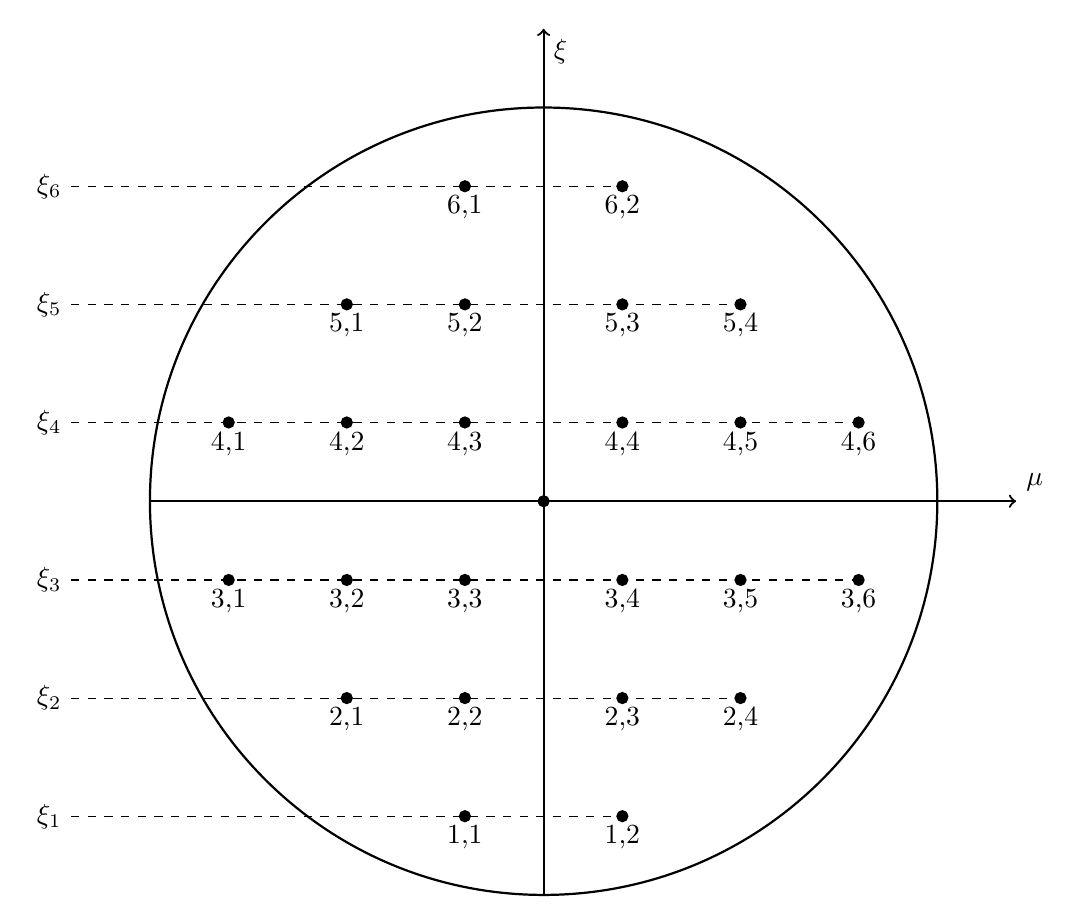
\begin{tikzpicture}

\draw[fill=black] (0,0) circle (2pt);
\draw[thick,->] (-5,0) -- (6,0) node[above right]{$\mu$};
\draw[thick,->] (0,-5) -- (0,6) node[below right]{$\xi$};
\draw[thick] (0,0) circle (5cm);

\draw[dashed] (-6,-4) node[left]{$\xi_1$} -- (1,-4);
\draw[dashed] (-6,-2.5) node[left]{$\xi_2$} -- (2.5,-2.5);
\draw[dashed] (-6,-1) node[left]{$\xi_3$} -- (4,-1);
\draw[dashed] (-6,1) node[left]{$\xi_4$} -- (4,1);
\draw[dashed] (-6,2.5) node[left]{$\xi_5$} -- (2.5,2.5);
\draw[dashed] (-6,4) node[left]{$\xi_6$} -- (1,4);

\draw[fill=black] (-4,-1) circle (2pt) node[below]{3,1};
\draw[fill=black] (-2.5,-1) circle (2pt) node[below]{3,2};
\draw[fill=black] (-1,-1) circle (2pt) node[below]{3,3};
\draw[fill=black] (-2.5,-2.5) circle (2pt) node[below]{2,1};
\draw[fill=black] (-1, -2.5) circle (2pt) node[below]{2,2};
\draw[fill=black] (-1,-4) circle (2pt) node[below]{1,1};

\draw[fill=black] (1,-1) circle (2pt) node[below]{3,4};
\draw[fill=black] (2.5,-1) circle (2pt) node[below]{3,5};
\draw[fill=black] (4,-1) circle (2pt) node[below]{3,6};
\draw[fill=black] (1, -2.5) circle (2pt) node[below]{2,3};
\draw[fill=black] (2.5,-2.5) circle (2pt) node[below]{2,4};
\draw[fill=black] (1,-4) circle (2pt) node[below]{1,2};

\draw[fill=black] (-4,1) circle (2pt) node[below]{4,1};
\draw[fill=black] (-2.5,1) circle (2pt) node[below]{4,2};
\draw[fill=black] (-1,1) circle (2pt) node[below]{4,3};
\draw[fill=black] (-2.5,2.5) circle (2pt) node[below]{5,1};
\draw[fill=black] (-1, 2.5) circle (2pt) node[below]{5,2};
\draw[fill=black] (-1,4) circle (2pt) node[below]{6,1};

\draw[fill=black] (1,1) circle (2pt) node[below]{4,4};
\draw[fill=black] (2.5,1) circle (2pt) node[below]{4,5};
\draw[fill=black] (4,1) circle (2pt) node[below]{4,6};
\draw[fill=black] (1, 2.5) circle (2pt) node[below]{5,3};
\draw[fill=black] (2.5,2.5) circle (2pt) node[below]{5,4};
\draw[fill=black] (1,4) circle (2pt) node[below]{6,2};

\end{tikzpicture}
\caption{Angular discretization showing $(\xi,\mu)$ pairs; adapted from \cite{Lewis_Comp_Methods_Neu_Trans}}
\label{fig:AngularDiscretization}
\end{figure}

One of the major challenges is handling the anglar derivative term. Lewis and Miller \cite{Lewis_Comp_Methods_Neu_Trans} describes an approximation for the partial derivative of the intensity with respect to $\omega$:
\begin{flalign}
- \frac{1}{r} \frac{\partial}{\partial \omega} \eta_{m,n} \psi_{n,m} \left(r,z \right) & = \frac{\alpha_{m+1/2}^n \psi_{n,m+1/2} (r,z) - \alpha_{m-1/2}^n \psi_{n,m-1/2} (r,z)}{r w_{n,m}}
\end{flalign}

\noindent where $\alpha_{m+1/2}^n$ and $\alpha_{m-1/2}^n$ are angular differencing coefficients, and $w_{n,m}$ is the angular quadrature weight. We substitute this into Equation \ref{eq:RZSNTransport},
\begin{multline}
\frac{\mu_{n,m}}{r} \frac{\partial}{\partial r} r \psi_{n,m} \left(r,z \right) + \xi_n \frac{\partial}{\partial z} \psi_{n,m} \left(r,z \right) \\
+ \frac{\alpha_{m+1/2}^n \psi_{m+1/2,n} (r,z) - \alpha_{m-1/2}^n \psi_{m-1/2,n} (r,z)}{r w_{n,m}} + \sigma_t \left(r,z \right) \psi_{n,m} \left(r,z \right) \\
= \frac{1}{4 \pi} \int_{4 \pi} \sigma_s \left(r,z \right) \psi \left(r,z, \vec{\Omega}^\prime \right) d \Omega^\prime + \frac{1}{4 \pi} S_0 \left(r,z \right)
\label{eq:RZSNADTransport}
\end{multline}

\noindent Here, we pause to notice that there are similarities and differences between our Cartesian discretization. The absorption term, axial derivative term, and right-hand-side are the same in both coordinate systems. The differences arise in the radial and angular derivative terms. 


After multiplying through by the radius $r$, the radial derivative term has a factor of $r$ inside the derivative. The angular derivative term is also new and does not resemble a mass matrix so MFEM will require additional modification.

Requiring Equation \ref{eq:RZSNADTransport} to satisfy the uniform infinite medium solution results in the condition,
\begin{flalign}
\alpha_{m+1/2}^n & = \alpha_{m-1/2}^n - \mu_{n,m} w_{n,m}
\label{eq:AlphaMinusMuW}
\end{flalign}

\iffalse
\begin{multline}
\int_{4 \pi} d \Omega \left[ \frac{\mu_{n,m}}{r} \frac{\partial}{\partial r} r \psi_{n,m} \left(r,z \right) + \frac{\alpha_{m+1/2}^n \psi_{m+1/2,n} (r,z) - \alpha_{m-1/2}^n \psi_{m-1/2,n} (r,z)}{r w_{n,m}} \right. \\
\left. + \xi_n \frac{\partial}{\partial z} \psi_{n,m} \left(r,z \right) \right] + \sigma_t \left(r,z \right) \phi \left(r,z \right) \\
= \sigma_s \left(r,z \right) \phi \left(r,z\right) + S_0 \left(r,z \right)
\end{multline}
\begin{multline}
\int_{4 \pi} d \Omega \left[ \frac{\mu_{n,m}}{r} \frac{\partial}{\partial r} r \psi_{n,m} \left(r,z \right) + \frac{\alpha_{m+1/2}^n \psi_{m+1/2,n} (r,z) - \alpha_{m-1/2}^n \psi_{m-1/2,n} (r,z)}{r w_{n,m}} \right. \\
\left. + \xi_n \frac{\partial}{\partial z} \psi_{n,m} \left(r,z \right) \right] = 0
\end{multline}

\noindent That is, the streaming term must equal zero because $\sigma_t = \sigma_a + \sigma_s$. Using the product rule,
\begin{multline}
\int_{4 \pi} d \Omega \left[\frac{\mu_{n,m}}{r} \left(\frac{\partial r}{\partial r} \psi_{n,m} + r \frac{\partial \psi_{n,m} (r,z)}{\partial r} \right) + \right. \\
\left. \frac{\alpha_{m+1/2}^n \psi_{m+1/2,n} (r,z) - \alpha_{m-1/2}^n \psi_{m-1/2,n} (r,z)}{r w_{n,m}} + \xi_n \frac{\partial}{\partial z} \psi_{n,m} \left(r,z \right) \right] = 0
\end{multline}
\begin{flalign}
\int_{4 \pi} d \Omega \left[\frac{\mu_{n,m}}{r} \psi_{n,m} + \frac{\alpha_{m+1/2}^n \psi_{m+1/2,n} (r,z) - \alpha_{m-1/2}^n \psi_{m-1/2,n} (r,z)}{r w_{n,m}} \right] & = 0 \\
\left(\frac{\mu_{n,m}}{r} + \frac{\alpha_{m+1/2}^n - \alpha_{m-1/2}^n}{r w_{n,m}} \right) \phi(r,z) & = 0
\end{flalign}

\noindent results in the condition,
\begin{flalign}
\alpha_{m+1/2}^n & = \alpha_{m-1/2}^n - \mu_{n,m} w_{n,m}
\label{eq:AlphaMinusMuW}
\end{flalign}
\fi

\noindent If $\alpha_{1/2}^n$ is known, then the remaining coefficients are uniquely determined. To find $\alpha_{1/2}^n$, we require that Equation \ref{eq:RZSNADTransport} satisfy the conservation equation (Eq. \ref{eq:RZTransport}).
%
\iffalse
Discretizing Equation \ref{eq:RZTransport} using discrete ordinates and summing over all directions (approximately integrating over all directions),
\begin{multline}
\sum_{n=1}^N \sum_{m=1}^{M_n} \frac{1}{r} \frac{\partial}{\partial r} r w_{n,m} \mu_{n,m} \psi_{n,m} \left(r,z \right) - \sum_{n=1}^N \sum_{m=1}^{M_n} \frac{1}{r} \frac{\partial}{\partial \omega} w_{n,m} \eta_{n,m} \psi_{n,m} \left(r,z \right) \\
+ \sum_{n=1}^N \sum_{m=1}^{M_n} \xi_n \frac{\partial}{\partial z} w_{n,m} \psi_{n,m} \left(r,z \right) + \sum_{n=1}^N \sum_{m=1}^{M_n} \sigma_t \left(r,z \right) \psi_{n,m} \left(r,z \right) \\
= \sum_{n=1}^N \sum_{m=1}^{M_n} w_{n,m} \frac{1}{4 \pi} \int_{4 \pi} \sigma_s \left(r,z \right) \psi \left(r,z, \vec{\Omega}^\prime \right) d \Omega^\prime + \sum_{n=1}^N \sum_{m=1}^{M_n} w_{n,m} \frac{1}{4 \pi} S_0 \left(r,z \right)
\end{multline}

\noindent Given that the sum of the weights is $\sum w = 4 \pi$,
\begin{multline}
\sum_{n=1}^N \sum_{m=1}^{M_n} \frac{1}{r} \frac{\partial}{\partial r} r w_{n,m} \mu_{n,m} \psi_{n,m} \left(r,z \right) - \sum_{n=1}^N \sum_{m=1}^{M_n} \frac{1}{r} \frac{\partial}{\partial \omega} w_{n,m} \eta_{n,m} \psi_{n,m} \left(r,z \right) \\
+ \sum_{n=1}^N \sum_{m=1}^{M_n} \xi_n \frac{\partial}{\partial z} w_{n,m} \psi_{n,m} \left(r,z \right) \\
= - \sum_{n=1}^N \sum_{m=1}^{M_n} \sigma_t \left(r,z \right) \psi_{n,m} \left(r,z \right) + \int_{4 \pi} \sigma_s \left(r,z \right) \psi \left(r,z, \vec{\Omega}^\prime \right) d \Omega^\prime +  S_0 \left(r,z \right)
\end{multline}

\noindent Multiplying Equation \ref{eq:RZSNADTransport} by weight $w_{n,m}$ and summing over all directions results in
\begin{multline}
\sum_{n=1}^N \sum_{m=1}^{M_n} w_{n,m} \frac{\mu_{n,m}}{r} \frac{\partial}{\partial r} r \psi_{n,m} \left(r,z \right) + \sum_{n=1}^N \sum_{m=1}^{M_n} w_{n,m} \frac{\alpha_{m+1/2}^n \psi_{m+1/2,n} (r,z) - \alpha_{m-1/2}^n \psi_{m-1/2,n} (r,z)}{r w_{n,m}} \\
+ \sum_{n=1}^N \sum_{m=1}^{M_n} w_{n,m} \xi_n \frac{\partial}{\partial z} \psi_{n,m} \left(r,z \right) + \sum_{n=1}^N \sum_{m=1}^{M_n} w_{n,m} \sigma_t \left(r,z \right) \psi_{n,m} \left(r,z \right) \\
= \sum_{n=1}^N \sum_{m=1}^{M_n} w_{n,m} \frac{1}{4 \pi} \int_{4 \pi} \sigma_s \left(r,z \right) \psi \left(r,z, \vec{\Omega}^\prime \right) d \Omega^\prime + \sum_{n=1}^N \sum_{m=1}^{M_n} w_{n,m} \frac{1}{4 \pi} S_0 \left(r,z \right)
\end{multline}

\noindent Then, to satisfy the condition,
\begin{multline}
- \sum_{n=1}^N \sum_{m=1}^{M_n} w_{n,m} \frac{1}{r} \frac{\partial}{\partial \omega} \eta_{n,m} \psi_{n,m} \left(r,z \right) \\
= \sum_{n=1}^N \sum_{m=1}^{M_n} w_{n,m} \frac{\alpha_{m+1/2}^n \psi_{m+1/2,n} (r,z) - \alpha_{m-1/2}^n \psi_{m-1/2,n} (r,z)}{r w_{n,m}}
\end{multline}
\begin{multline}
- \sum_{n=1}^N \sum_{m=1}^{M_n} w_{n,m} \left(\frac{\partial \eta_{n,m}}{\partial \omega} \psi_{n,m} \left(r,z \right) + \eta_{n,m} \frac{\partial \psi_{n,m} \left(r,z \right)}{\partial \omega} \right) \\
= \sum_{n=1}^N \sum_{m=1}^{M_n} \left(\alpha_{m+1/2}^n \psi_{m+1/2,n} (r,z) - \alpha_{m-1/2}^n \psi_{m-1/2,n} (r,z) \right)
\end{multline}

\noindent If $\int_{2 \pi} d \omega \frac{\partial}{\partial \omega} \eta \psi = 0$, then
\begin{flalign}
\sum_{m=1}^{M_n} \left(\alpha_{m+1/2}^n \psi_{m+1/2,n} (r,z) - \alpha_{m-1/2}^n \psi_{m-1/2,n} (r,z) \right) & = 0 \\
\alpha_{1/2}^n \psi_{1/2,n} (r,z) - \alpha_{M_n + 1/2}^n \psi_{M_n + 1/2,n} (r,z) & = 0
\end{flalign}
\fi
%
Given a quadrature set with an even number of $\mu_{n,m}$ values, setting $\alpha_{1/2}^n = 0$ results in $\alpha_{M_n + 1/2}^n = 0$ per Equation \ref{eq:AlphaMinusMuW} and the conservation equation is satisfied.

\iffalse
 for any value of $\psi_{1/2,n} (r,z)$ and $\psi_{M_n + 1/2,n} (r,z)$.
\fi

A relationship between $\psi_{n,m}$, $\psi_{n,m+1/2}$, and $\psi_{n,m-1/2}$ must be established. A weighted diamond difference scheme has been established by Morel and Montry \cite{MorelAnalysisEliminationFluxDip},
\begin{flalign}
\psi_{n,m} (r,z) & = \tau_{n,m} \psi_{n,m+1/2} + \left(1- \tau_{n,m} \right) \psi_{n,m-1/2}
\label{eq:LinearAngularFluxTau}
\end{flalign}

\noindent where $\tau_{n,m}$ linearly interpolates $\mu$:
\begin{flalign}
\tau_{n,m} & = \frac{\mu_{n,m} - \mu_{n,m-1/2}}{\mu_{n,m+1/2} - \mu_{n,m-1/2}}
\label{eq:LinearTau}
\end{flalign}

\noindent with
\begin{flalign}
\mu_{n,m+1/2} & = \sqrt{1 - \xi_n^2} \cos \left(\varphi_{n,m+1/2} \right) \\
\varphi_{n,m+1/2} & = \varphi_{n,m-1/2} + \pi \frac{w_{n,m}}{w_n} \\
w_n & = \sum_{m=1}^{M_n} w_{n,m}
\end{flalign}


We take Equation \ref{eq:RZSNADTransport}, multiply through by $r$ and perform a product rule on the radial derivative term,
\begin{multline}
\mu_{n,m} \left[\psi_{n,m} \left(r,z \right) + r \frac{\partial}{\partial r}  \psi_{n,m} \left(r,z \right) \right] + r \xi_n \frac{\partial}{\partial z} \psi_{n,m} \left(r,z \right) \\
+ \frac{\alpha_{m+1/2}^n \psi_{m+1/2,n} (r,z) - \alpha_{m-1/2}^n \psi_{m-1/2,n} (r,z)}{w_{n,m}} + r \sigma_t \left(r,z \right) \psi_{n,m} \left(r,z \right) \\
= \frac{r}{4 \pi} \int_{4 \pi} \sigma_s \left(r,z \right) \psi \left(r,z, \vec{\Omega}^\prime \right) d \Omega^\prime + \frac{r}{4 \pi} S_0 \left(r,z \right).
\end{multline}
%
We solve Equation \ref{eq:LinearAngularFluxTau} for $\psi_{n,m+1/2}$, perform a substitution, and move the known quantities to the right-hand-side,
\begin{multline}
\mu_{n,m} r \frac{\partial}{\partial r}  \psi_{n,m} \left(r,z \right) + r \xi_n \frac{\partial}{\partial z} \psi_{n,m} \left(r,z \right) + \mu_{n,m} \psi_{n,m} \left(r,z \right) \\
+ \frac{\alpha_{m+1/2}^n}{\tau_{n,m} w_{n,m}} \psi_{n,m}(r,z) + r \sigma_t \left(r,z \right) \psi_{n,m} \left(r,z \right) \\
= \frac{r}{4 \pi} \int_{4 \pi} \sigma_s \left(r,z \right) \psi \left(r,z, \vec{\Omega}^\prime \right) d \Omega^\prime + \frac{r}{4 \pi} S_0 \left(r,z \right) \\
+ \left(\frac{1-\tau_{n,m}}{\tau_{n,m}} \frac{\alpha_{m+1/2}^n}{w_{n,m}} + \frac{\alpha_{m-1/2}^n}{w_{n,m}} \right) \psi_{n,m-1/2}(r,z).
\label{eq:RZSNTransport}
\end{multline}

Given a level-symmetric quadrature set, all of the $\alpha_{n,m \pm 1/2}^n$ and $\tau_{n,m}$ values can be computed. We solve the starting direction equation to obtain $\psi_{n,1/2}$. That is, we solve the \XY\ system for directions $\vec{\Omega}_{n,1/2}$,
\begin{flalign}
\vec{\Omega}_{n,1/2} \vd \grad \psi_{n,1/2} + \sigma_t \psi_{n,1/2} & = \frac{1}{4 \pi} \sigma_s \phi + \frac{1}{4 \pi} S_0
\end{flalign}

There is an alternate angular discretization method developed by Warsa and Prinja \cite{WarsaAngularQuadrature}. Instead of finding an approximation for the angular derivative, they perform a product rule:
\begin{flalign}
\frac{\partial \psi}{\partial \omega} & \equiv \frac{\partial \mu}{\partial \omega} \frac{\partial \psi}{\partial \mu}
\end{flalign}
%
Since,
\begin{flalign}
\frac{\partial \mu}{\partial \omega} & \equiv - \xi,
\end{flalign}
%
The angular derivative can be written
\begin{flalign}
\frac{\partial \psi}{\partial \omega} & \equiv - \xi \frac{\partial \psi}{\partial \mu}
\end{flalign}
%
Here, an approximation for the $\mu$-derivative must be established.


%%%%%%%%%%%%%%%%%%%%%%%%%%%%%%%%%%%%%%%
\subsection{Spatial Discretization}
The finite element discretization is performed here. The methodology is similar to the Cartesian geometry. First, we subdivide a problem domain using a spatial mesh. Then, we multiply Equation \ref{eq:RZSNTransport} by a test function and integrate over the volume of a single mesh zone,
\begin{multline}
\left(r \vec{\Omega}_{n,m} \vd \grad \psi_{n,m}, v_i \right)_{\mathbb{D}} + \left(\mu_{n,m} \psi_{n,m}, v_i \right)_{\mathbb{D}} \\
+ \left(\frac{\alpha_{m+1/2}^n}{\tau_{n,m} w_{n,m}} \psi_{n,m}, v_i \right)_{\mathbb{D}} + \left(r \sigma_t\psi_{n,m}, v_i \right)_{\mathbb{D}} \\
= \left(\frac{r}{4 \pi} \int_{4 \pi} \sigma_s \psi d \Omega^\prime, v_i \right)_{\mathbb{D}} + \left(\frac{r}{4 \pi} S_0, v_i \right)_{\mathbb{D}} \\
+ \left(\left(\frac{1-\tau_{n,m}}{\tau_{n,m}} \frac{\alpha_{m+1/2}^n}{w_{n,m}} + \frac{\alpha_{m-1/2}^n}{w_{n,m}} \right) \psi_{n,m-1/2}, v_i \right)_{\mathbb{D}},
\end{multline}
%
where the Cartesian gradient operator is used and the inner product notation,
\begin{flalign}
(a,b)_{\mathbb{D}} & \equiv \int_{\mathbb{D}} a b,
\end{flalign}
%
is used. We perform an integration by parts,
\begin{multline}
\left(r \vec{\Omega}_{n,m} \vd \hat{n} \psi_{n,m}, v_i \right)_{\partial \mathbb{D}} - \left(r \psi_{n,m}, \vec{\Omega}_{n,m} \vd \grad v_i \right)_{\mathbb{D}} + \left(\mu_{n,m} \psi_{n,m}, v_i \right)_{\mathbb{D}} \\
+ \left(\frac{\alpha_{m+1/2}^n}{\tau_{n,m} w_{n,m}} \psi_{n,m}, v_i \right)_{\mathbb{D}} + \left(r \sigma_t\psi_{n,m}, v_i \right)_{\mathbb{D}} \\
= \left(\frac{r}{4 \pi} \int_{4 \pi} \sigma_s \psi d \Omega^\prime, v_i \right)_{\mathbb{D}} + \left(\frac{r}{4 \pi} S_0, v_i \right)_{\mathbb{D}} \\
+ \left(\left(\frac{1-\tau_{n,m}}{\tau_{n,m}} \frac{\alpha_{m+1/2}^n}{w_{n,m}} + \frac{\alpha_{m-1/2}^n}{w_{n,m}} \right) \psi_{n,m-1/2}, v_i \right)_{\mathbb{D}},
\end{multline}
%
to obtain our angular and spatially discretized \RZ\ transport equation.




%%%%%%%%%%%%%%%%%%%%%%%%%%%%%%%%%%%%%%%
\subsection{Lumping}

%%%%%%%%%%%%%%%%%%%%%%%%%%%%%%%%%%%%%%%
\subsection{Diffusion Synthetic Acceleration}



%%%%%%%%%%%%%%%%%%%%%%%%%%%%%%%%%%%%%%%
\subsection{Symmetry Preservation}

%%%%%%%%%%%%%%%%%%%%%%%%%%%%%%%%%%%%%%%
\subsection{Other}

%%%%%%%%%%%%%%%%%%%%%%%%%%%%%%%%%%%%%%%
\subsection{Reflecting Boundary Conditions}

To incorporate reflecting boundary conditions, we will ``guess'' the incident angular fluxes, update them with outgoing angular fluxes from the previous iteration, and adapt a convergence criterion for those fluxes. Along the z-axis, the reflection for direction $\vec{\Omega} = (\mu, \eta, \xi)$ is $\vec{\Omega}_R = (-\mu, \eta, \xi)$.




%\bibliographystyle{apalike}
%\bibliography{Thesis_bib}

\end{document}
